\documentclass{beamer}
\usefonttheme{structuresmallcapsserif}
\usepackage{graphicx}
\usepackage{bussproofs}
\usepackage{amssymb}
\usepackage{amsfonts}
\usepackage{amsthm}
\usepackage{amsmath}
\usepackage{tikz}
\usepackage{tikz-cd}
\usetheme{Darmstadt}
\setbeamertemplate{footline}[frame number]
\AtBeginSection[]
{
\begin{frame}
\frametitle{Table of Contents}
\tableofcontents[currentsection]
\end{frame}
}

\title{KW: la logica della dimostrabilità}
\author{Giorgia Dal Prà}
\institute{Alma Mater Studiorum -- Univesità di Bologna}
\date{6 Maggio 2024}
\begin{document}

\begin{frame}
\maketitle   
\end{frame}

\begin{frame}{Indice}
    \tableofcontents
\end{frame}

\section{Storia di KW}
\begin{frame}{Storia di KW}
\begin{thebibliography}{1}
    \bibitem{} Gödel, K., 1933, “Eine Interpretation des intuitionistischen Aussagenkalküls,” \textit{Ergebnisse eines Mathematischen Kolloquiums}, 4: 39–40; translation “An Interpretation of the Intuitionistic  Propositional Calculus,” in K. Gödel, \textit{Collected Works}
\end{thebibliography}
 G\"odel 1933 suggerisce \textit{en passant} di interpretare l'essere dimostrabile come un operatore modale.\newline\newline
KW è una logica modale che ben rappresenta la dimostrabilità nell'aritmetica di Peano (PA).

\end{frame}



\section{Proprietà di KW}
\begin{frame}{Il sistema assiomatico di KW}
La logica KW è definita dagli assiomi:
\begin{exampleblock}{}
    \begin{itemize}
        \item Tutte le tautologie\qquad\qquad\qquad\qquad\qquad\qquad ($Taut$)
        \item $\Box(A \to B) \to (\Box A \to \Box B)$\qquad\qquad\qquad\qquad\quad ($K$)
        \item $\Box (\Box A \to A) \to \Box A$\qquad\qquad\qquad\qquad\qquad\qquad ($W$)
        \item $\Diamond A \leftrightarrow \neg\Box\neg A$\qquad\qquad\qquad\qquad\qquad\qquad\qquad ($def_\Diamond$)
    \end{itemize}
\end{exampleblock}

e dalle regole di inferenza:
\begin{exampleblock}{}
        \begin{prooftree}
        \AxiomC{$A\rightarrow B$}
        \AxiomC{$A$}
        \RightLabel{$MP$}
        \BinaryInfC{$B$}
    \end{prooftree}
    \begin{prooftree}
        \AxiomC{$A$}
        \RightLabel{$N$}
        \UnaryInfC{$\Box A$}
    \end{prooftree}
\end{exampleblock}

\end{frame}




\begin{frame}{Corrispondenza e validità}
\newtheorem{teorema}{Teorema}
\begin{teorema}[ordine dualmente ben fondato]
Lo schema W è valido su una struttura se e solo se essa ha una relazione d’accessibilità dualmente ben fondata e transitiva:
\begin{center}
    $\mathcal{F} \models \Box(\Box A \to A) \to \Box A$ \textit{sse} $\mathcal{F}\rhd \textit{dualmente ben fondato}$
\end{center}

\end{teorema}
\theoremstyle{definition}
\newtheorem{defn}{Definizione}
\begin{defn}
Una relazione $\mathcal{R}$ è un \textit{ordine dualmente ben fondato} sse $\mathcal{R}$ è irriflessiva, transitiva e non esistono catene infinite ascendenti, ovvero non esistono $\mathcal{R}$-successioni infinite: $x_{0}\mathcal{R}x_{1}\mathcal{R}x_{2}\mathcal{R}x_{3}\mathcal{R}$...
\end{defn}
\end{frame}





\begin{frame}{Validità}
Dal Teorema 1 segue:
\newtheorem{teorema}
\begin{teorema}
KW è valida sulla classe delle strutture irriflesive, transitive e prive di $\mathcal{R}$-catene infinite ascendenti. In particolare KW è valida rispetto alla classe degli ordini parziali stretti finiti.
\end{teorema}
\end{frame}






\begin{frame}{Teorema $\vdash_{KW} $  $\Box B \to \Box\Box B$}
\begin{proof}
    \begin{enumerate}
        \item $\vdash_{KW} B \to ((\Box B \wedge \Box\Box B) \to (B \wedge \Box B))\quad\qquad\qquad\text{Taut}$
        \item $\vdash_{KW} B \to (\Box (B \wedge \Box B) \to (B \wedge \Box B))\quad\qquad\quad\text{K(1), Taut [1]}$
        \item $\vdash_{KW} \Box B \to \Box(\Box (B \wedge \Box B) \to (B \wedge \Box B))\qquad\qquad\text{RM [2]}$
        \item $\vdash_{KW} \Box(\Box (B \wedge \Box B) \to (B \wedge \Box B)) \to \Box(B \wedge \Box B))\quad\text{W}$
        \item $\vdash_{KW} \Box B \to \Box(B \wedge \Box B)\qquad\qquad\qquad\qquad\qquad\quad\text{Taut [3,4]}$
        \item $\vdash_{KW} \Box B \to \Box B \wedge \Box\Box B\qquad\qquad\qquad\qquad\qquad\text{K(1), Taut [5]}$
        \item $\vdash_{KW} \Box B \to \Box\Box B\qquad\qquad\qquad\qquad\qquad\qquad\qquad\text{Taut [6]}$
    \end{enumerate}
\end{proof}

\end{frame}





\begin{frame}{Teoremi e non teoremi di KW}
\begin{exampleblock}{Sono teoremi di KW:}
    \begin{itemize}
        \item $((\Box A \to A) \wedge \Box(\Box A \to A)) \to A$
        \item $\Box(\Box\bot\to\bot)\to\Box\bot$
        \item $\Diamond \top \to \neg\Box\Diamond\top$
        \item $\Diamond \top \to \Diamond\Box\bot$
        \item $\Box\bot\leftrightarrow\Box\Diamond\top$
    \end{itemize}
\end{exampleblock}
\begin{alertblock}{Non sono teoremi di KW:}
    \begin{itemize}
        \item $\Box A \leftrightarrow A$
        \item $\Diamond\top$
        \item $\neg\Box\bot$
        \item $\Box\Diamond\top$
    \end{itemize}
\end{alertblock}

\end{frame}





\begin{frame}{Completezza di KW}
\newtheorem{teorema}
\begin{teorema}
La logica KW è completa rispetto agli ordini parziali stretti finiti.
\end{teorema}
\begin{teorema}
La logica KW non è fortemente completa, ovvero non vale che:
\[
\Gamma \vdash_{KW} B\quad sse\quad \Gamma \models_{KW} B
\]
\end{teorema}
\begin{teorema}
La logica KW non è canonica.
\end{teorema}
\end{frame}


\section{L'aritmetica di Peano}
\begin{frame}{Aritmetica di Peano}

    \begin{itemize}
        \item[(PA1)] $\forall x \neg (S(x)=0)$
        \item[(PA2)] $\forall x \forall y (S(x)=S(y)\rightarrow x=y)$
        \item[(PA3)] $\forall x (x+0=x)$
        \item[(PA4)] $\forall x \forall y (x+S(y)=S(x+y))$
        \item[(PA5)] $\forall x (x\cdot 0=0)$
        \item[(PA6)] $\forall x (x\cdot S(y)=(x\cdot y)+x)$
        \item[(PA7)] $\forall \vec{x} [(A(0,\vec{x})\land \forall y (A(y,\vec{x})\rightarrow A(S(y),\vec{x})))\rightarrow\forall y A(y,\vec{x})]$
    \end{itemize}

\end{frame}





\begin{frame}{Gödelizzazione}

Deriviamo il numero di G\"odel della formula $\forall x (x=x)$:
\begin{figure}
    \centering
    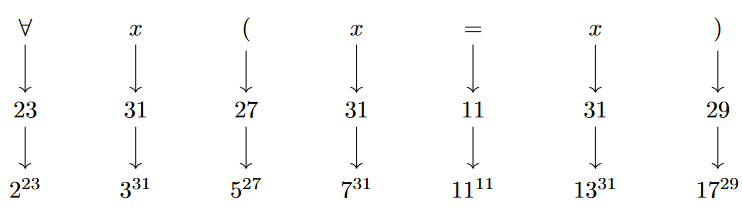
\includegraphics[scale=0.7]{godel.png}
    \caption{Esempio di calcolo del numero di G\"odel}
    \label{fig:enter-label}
\end{figure}



\end{frame}

\section{$Teor_{PA}(x)$ e KW}
\begin{frame}{Il predicato $Teor_{PA}(x)$} 
Sia $prova(n,m)$ la relazione che intercorre tra due numeri naturali $n$ e $m$ quando $n$ è il numero di Gödel di una dimostrazione di una formula di numero di Gödel $m$. Si dimostra che tale relazione è fortemente rappresentabile nell’aritmetica (formale) PA, ovvero che esiste una formula $Dim(x,y)$ di PA tale che per ogni $n$ ed $m$:
\begin{center}
    $PA \vdash Dim(\overline{n},\overline{m})$ se vale $prova (n, m)$

    $PA \vdash \neg Dim(\overline{n},\overline{m})$ se vale $non$ $prova (n, m)$
\end{center}
\begin{defn}
   \begin{center}
   $Teor_{PA}(x)$ sse $PA \vdash \exists y Dim(y,x)$
   \end{center}
\end{defn}
\end{frame}

\begin{frame}{Proprietà di $Teor_{PA}(x)$}
Il predicato unario $Teor_{PA}(x)$ gode delle seguenti proprietà:
\begin{exampleblock}{}
    \begin{itemize}
  \item[T1] $PA \vdash A$ solo se $PA \vdash Teor_{PA}(\overline{A})$;
  \item[T2] $PA \vdash Teor_{PA}(\overline{A}) \wedge Teor_{PA}(\overline{A\to B}) \to Teor_{PA}(\overline{B})$;
  \item[T3] $PA \vdash Teor_{PA}(\overline{A}) \to Teor_{PA}(\overline{Teor_{PA}(\overline{A})})$.
\end{itemize}
\end{exampleblock}
\end{frame}

\begin{frame}{Teorema di Löb}
Nel 1952 Leon Henkin pose una questione relativamente agli enunciati che esprimono la propria dimostrabilità, ovverro tali che $PA \vdash Teor_{PA}(\overline{A}) \leftrightarrow A$. Come sappiamo dal primo teorema di incompletezza gli enunciati che esprimono la propria indimostrabilità, ovverto tali che $PA \vdash \neg Teor_{PA}(\overline{A}) \leftrightarrow A$, non sono dimostrabili, ma sono veri.

Löb dimostra che il predicato $Teor_{PA}(x)$ gode della sequente properietà:
\begin{exampleblock}{}
\begin{itemize}
\item[T4] 
\begin{center}
$PA \vdash Teor_{PA}(\overline{A}) \to A$ solo se $PA \vdash A$  
\end{center}
\end{itemize}
\end{exampleblock}
Una versione formalizzata:
\begin{center}
    $PA \vdash Teor_{PA}(\overline{Teor_{PA}(\overline{A})} \to A) \to Teor_{PA}(\overline{A})$
\end{center}
\end{frame}


\begin{frame}{Realizzazione e teorema di Solovay}
Sia $\tau$ una funzione di traduzione dall’insieme delle variabili enunciative $\Phi$ a enunciati di PA, tale che:
\begin{itemize}
  \item $\tau(\bot)=\bot$;
  \item $\tau(A\to B)=\tau(A) \to \tau(B)$
  \item $\tau(\Box A) = Teor_{PA}(\tau(A))$
\end{itemize}

 \begin{teorema}[Teorema di Solovay, 1976]
   \begin{center}
        $\vdash_{KW}A$ sse per ogni traduzione $\tau$, $PA \vdash \tau(A)$
   \end{center} 
 \end{teorema}
\end{frame}



\section{Il secondo teorema di incompletezza}
\begin{frame}{2° teorema di Gödel via teorema di Löb}
\begin{block}{}
    Se $T$ è gödeliana e consistente, allora $\not\vdash CON_T$.
\end{block}
\begin{proof}
    Supponiamo per assurdo che $CON_T$, allora
    \begin{enumerate}
        \item $T\vdash \neg Teor_{PA}(\overline{\bot})$
        \item $T\vdash Teor_{PA}(\overline{\bot}) \to \bot \quad\qquad\quad\quad\qquad\quad\quad\qquad\text{Duns Scoto}$
        \item $T\vdash \bot \quad\qquad\quad\quad\qquad\quad\quad\qquad\quad\quad\qquad\quad\text{teorema di Löb}$
    \end{enumerate}
    Quindi T è inconsistente, contrariamente all’ipotesi.
\end{proof}

\end{frame}



\begin{frame}{Alcune proprietà metateoriche di PA}
\begin{exampleblock}{}
    \begin{itemize}
        \item $\neg Teor_{PA}(\overline{\bot})$
        \item $Teor_{PA}(\overline{\neg Teor_{PA}(\overline{\bot})})$
        \item $\neg Teor_{PA}(\overline{\bot})\to \neg Teor_{PA}(\overline{\neg Teor_{PA}(\overline{\bot})})$
        \item $Teor_{PA}(\overline{\neg Teor_{PA}(\overline{\bot})\to \neg Teor_{PA}(\overline{\neg Teor_{PA}(\overline{\bot})})})$
    \end{itemize}
\end{exampleblock}

\end{frame}


\end{document}




